% **************************************************
% Document Class Definition
% **************************************************
\documentclass[%
    paper=A4,               % paper size --> A4 is default in Germany
    twoside=true,           % onesite or twoside printing
    openright,              % doublepage cleaning ends up right side
    parskip=half,           % spacing value / method for paragraphs
    chapterprefix=true,     % prefix for chapter marks
    11pt,                   % font size
    headings=normal,        % size of headings
    bibliography=totoc,     % include bib in toc
    listof=totoc,           % include listof entries in toc
    titlepage=on,           % own page for each title page
    captions=tableabove,    % display table captions above the float env
    chapterprefix=false,    % do not display a prefix for chapters
    appendixprefix=false,    % but display a prefix for appendix chapter
    draft=false,            % value for draft version
]{scrreprt}%


% **************************************************
% Setup YOUR thesis document in this file !
% **************************************************
% !TEX root = proposal.tex


% **************************************************
% Files' Character Encoding
% **************************************************
\PassOptionsToPackage{utf8}{inputenc}
\usepackage{inputenc}


% **************************************************
% Information and Commands for Reuse
% **************************************************
\newcommand{\thesisTitle}{Answering Causal Questions \texorpdfstring{\\}{} with Reinforcement Learning}
\newcommand{\thesisName}{Lukas Blübaum}
\newcommand{\thesisSubject}{Proposal}
\newcommand{\thesisDate}{\today}
\newcommand{\thesisVersion}{Proposal}

\newcommand{\thesisFirstReviewer}{Prof. Dr. Axel-Cyrille Ngonga Ngomo}
\newcommand{\thesisFirstReviewerUniversity}{\protect{Paderborn University}}
\newcommand{\thesisFirstReviewerDepartment}{Department of Computer Science}

\newcommand{\thesisSecondReviewer}{Jun.-Prof. Dr. Sebastian Peitz}
\newcommand{\thesisSecondReviewerUniversity}{\protect{Paderborn University}}
\newcommand{\thesisSecondReviewerDepartment}{Department of Computer Science}

\newcommand{\thesisFirstSupervisor}{Dr. Stefan Heindorf}
%\newcommand{\thesisSecondSupervisor}{John Smith}

\newcommand{\thesisUniversity}{\protect{Paderborn University}}
\newcommand{\thesisUniversityDepartment}{Faculty for Computer Science, Electrical Engineering and Mathematics}
\newcommand{\thesisUniversityInstitute}{Department of Computer Science}
\newcommand{\thesisUniversityGroup}{DICE Research Group}
\newcommand{\thesisUniversityCity}{Paderborn}
\newcommand{\thesisUniversityStreetAddress}{Warburger Straße 100}
\newcommand{\thesisUniversityPostalCode}{33098}


% **************************************************
% Debug LaTeX Information
% **************************************************
%\listfiles


% **************************************************
% Load and Configure Packages
% **************************************************
\usepackage[english]{babel} % babel system, adjust the language of the content
\PassOptionsToPackage{% setup clean thesis style
    figuresep=colon,%
    hangfigurecaption=false,%
    hangsection=true,%
    hangsubsection=true,%
    sansserif=false,%
    configurelistings=true,%
    colorize=full,%
    colortheme=bluemagenta,%
    configurebiblatex=true,%
    bibsys=biber,%
    bibfile=bib-refs,%
    bibstyle=alphabetic,%
    bibsorting=nty,%
}{cleanthesis}
\usepackage{cleanthesis}

\hypersetup{% setup the hyperref-package options
    pdftitle={\thesisTitle},    %   - title (PDF meta)
    pdfsubject={\thesisSubject},%   - subject (PDF meta)
    pdfauthor={\thesisName},    %   - author (PDF meta)
    plainpages=false,           %   -
    colorlinks=false,           %   - colorize links?
    pdfborder={0 0 0},          %   -
    breaklinks=true,            %   - allow line break inside links
    bookmarksnumbered=true,     %
    bookmarksopen=true          %
}


% **************************************************
% OWN PACKAGES
% **************************************************

\usepackage{pgfgantt}

\usepackage{tikz}
\usetikzlibrary{shapes, arrows, arrows.meta, calc}
\usepackage{amsmath,amssymb}
\usepackage{booktabs}
\usepackage{svg}
\usepackage[linesnumbered]{algorithm2e}

\usepackage{xcolor}
\newcommand{\todo}[2][]{\textcolor{red}{TODO\@: #2}}



% **************************************************
% COLORS
% **************************************************

\definecolor{tab20darkblue}{HTML}{4e79a7}
\definecolor{tab20darkgreen}{HTML}{59a14f}
\definecolor{tab20darkred}{HTML}{e15759}
\definecolor{tab20darkorange}{HTML}{f28e2b}
\definecolor{tab20darkturquoise}{HTML}{499894}
\definecolor{tab20darkgray}{HTML}{79706e}
\definecolor{tab20darkbrown}{HTML}{9d7660}
\definecolor{tab20darkpurple}{HTML}{b07aa1}
\definecolor{tabl20lighgreen}{HTML}{8cd17d}
\definecolor{tab20lightblue}{HTML}{a0cbd8}


\definecolor{newgreen}{HTML}{148f77}
\definecolor{brass}{HTML}{E1C16E}


% **************************************************
% Document CONTENT
% **************************************************
\begin{document}

% uncomment the following command to fill up pages with
% whitespace instead of aligning the first and last lines
% of a page (see \raggedbottom vs. \flushbottom)
%\raggedbottom

% --------------------------
% rename document parts
% --------------------------
%\renewcaptionname{ngerman}{\figurename}{Abb.}
%\renewcaptionname{ngerman}{\tablename}{Tab.}
\renewcaptionname{english}{\figurename}{Fig.}
\renewcaptionname{english}{\tablename}{Tab.}

% --------------------------
% Front matter
% --------------------------
\pagenumbering{roman}			% roman page numbing (invisible for empty page style)
\pagestyle{empty}				% no header or footers
% !TEX root = my-thesis.tex
%
% ------------------------------------  --> cover title page
\begin{titlepage}
	\pdfbookmark[0]{Cover}{Cover}
	\flushright
	\hfill
	\vfill
	{\LARGE\thesisTitle \par}
	\rule[5pt]{\textwidth}{.4pt} \par
	{\Large\thesisName}
	\vfill
	\textit{\large\thesisDate} \\
	Version: \thesisVersion
\end{titlepage}


% ------------------------------------  --> main title page
\begin{titlepage}
	\pdfbookmark[0]{Titlepage}{Titlepage}
	\tgherosfont
	\centering

	%{\Large \thesisUniversity} \\[4mm]
	
\includegraphics[width=10cm]{figures/uni-logo} \\[2mm]
	\textsf{\thesisUniversityDepartment} \\
	\textsf{\thesisUniversityInstitute} \\
	\textsf{\thesisUniversityGroup} \\

	\vfill
	{\large \thesisSubject} \\[5mm]
	{\LARGE \color{ctcolortitle}\textbf{\thesisTitle} \\[10mm]}
	{\Large \thesisName} \\

	\vfill
	\begin{minipage}[t]{.27\textwidth}
		\raggedleft
		\textit{1. Reviewer}
	\end{minipage}
	\hspace*{15pt}
	\begin{minipage}[t]{.65\textwidth}
		{\Large \thesisFirstReviewer} \\
	  	{\small \thesisFirstReviewerDepartment} \\[-1mm]
		{\small \thesisFirstReviewerUniversity}
	\end{minipage} \\[5mm]
	\begin{minipage}[t]{.27\textwidth}
		\raggedleft
		\textit{2. Reviewer}
	\end{minipage}
	\hspace*{15pt}
	\begin{minipage}[t]{.65\textwidth}
		{\Large \thesisSecondReviewer} \\
	  	{\small \thesisSecondReviewerDepartment} \\[-1mm]
		{\small \thesisSecondReviewerUniversity}
	\end{minipage} \\[10mm]
	\begin{minipage}[t]{.27\textwidth}
		\raggedleft
		\textit{Supervisor}
	\end{minipage}
	\hspace*{15pt}
	\begin{minipage}[t]{.65\textwidth}
		\thesisFirstSupervisor\ %and \thesisSecondSupervisor
	\end{minipage} \\[10mm]

	\thesisDate \\

\end{titlepage}


% ------------------------------------  --> lower title back for single page layout
\hfill
\vfill
{
	\small
	\textbf{\thesisName} \\
	%\textit{\thesisTitle} \\
	\textit{Answering Causal Questions with Reinforcement Learning} \\
	\thesisSubject, \thesisDate \\
	Reviewers: \thesisFirstReviewer\ and \thesisSecondReviewer \\
	Supervisor: \thesisFirstSupervisor\ \\[1.5em]%and \thesisSecondSupervisor \\[1.5em]
	\textbf{\thesisUniversity} \\
	\textit{\thesisUniversityGroup} \\
	\thesisUniversityInstitute \\
	\thesisUniversityDepartment \\
	\thesisUniversityStreetAddress \\
	\thesisUniversityPostalCode\ \thesisUniversityCity
}
		% INCLUDE: all titlepages
\cleardoublepage

\pagestyle{plain}				% display just page numbers
%%\vspace*{\fill}
\chapter*{Abstract}
Causal questions seek to determine whether there exists a causal relationship 
between different events or phenomena. 
Specifically, they often aim to understand the underlying causes of an effect or what kind of effects a particular cause might have in the future.
Causal questions are important for various use cases, for example, in virtual assistants or search engines.
However, many current approaches to causal question answering cannot provide explanations or verifications for their answers. 
Additionally, the approaches were often missing 
large-scale datasets of causal relations.
In this thesis, we explore the application of reinforcement learning on CauseNet, a large-scale causal knowledge graph, to answer binary causal questions inspired by the successful application of reinforcement learning in knowledge graph tasks, such as link prediction and fact-checking.
We introduce an Actor-Critic based agent which learns to search through the graph to answer binary causal questions.
Additionally, we bootstrap the agent with a supervised learning procedure and adapt an existing reward shaping strategy to deal 
with large action spaces and sparse rewards.
Our evaluation shows that our agent successfully prunes the search to answer binary causal questions efficiently.
Moreover, our ablation study indicates that the supervised learning strategy provides a strong foundation upon which the agent can improve.
Finally, we demonstrate how the paths learned by the agent can be used to explain causal relations, to indicate the specific mechanisms by which a cause produces an effect.
%\vspace*{\fill}		% INCLUDE: the abstracts (english and german)
\cleardoublepage
%
%\input{content/acknowledgement} % INCLUDE: acknowledgement
\cleardoublepage
%
\currentpdfbookmark{\contentsname}{toc}
\setcounter{tocdepth}{2}		% define depth of toc
\tableofcontents				% display table of contents
\cleardoublepage

% --------------------------
% Body matter
% --------------------------
\pagenumbering{arabic}			% arabic page numbering
\setcounter{page}{1}			% set page counter
\pagestyle{scrheadings}			% header and footer style

%% Uncomment the following lines using the \part command
%% to add part sections
%\part{Example Part}
% !TEX root = my-thesis.tex
%
\chapter{Introduction}
\label{ch:introduction}

Causal question answering addresses the problem of determining the causal relations between given causes and effects~\cite{KayeshCausalTransfer2020, DalalCausalQAEnhancing2021}. This could involve examining whether a causal relation exists or how a causal relation can be explained.
For example, causal questions like \textit{``Does pneumonia cause anemia?''} ask for the validity of a causal relation.
Instead, more complicated questions like \textit{``How does pneumonia cause death?''} might ask for an explanation of a causal relation. 
Nowadays, the necessity to answer causal questions arises in various domains. For example, users often seek answers to causal questions from virtual assistants like Alexa or from search engines~\cite{Nguyen2016MSMARCO, Heindorf2020Causenet}. Similarly, causal questions and explanations for causal relations are important for argumentation~\cite{Walton2007Dialog, Habernal2018Argumentation} and automated decision-making~\cite{HassanzadeshCausalQA2019, KayeshCausalTransfer2020, Heindorf2020Causenet}.
When possible, tracing the causality chain that led to an answer can provide further insights and a deeper understanding of the causal relationship in question.


%\begin{itemize}
%    \item example
    %\item learned by humans through everyday life, still often not true or justified (CauseNet paper)
    %\item maybe historic context, aristotle, socrates
    %\item Important because many causal questions (asked by search engine users, c.f., MS MARCO), alexa, necessary for argumentation, decision making
    %\item judea pearl, the book of why -- correlation -> causality
%\end{itemize}


Therefore, the literature started to introduce approaches for causal question answering~\cite{SharpCausalQAEmbeddings2016, HassanzadeshCausalQA2019, KayeshCausalTransfer2020, DalalCausalQAISWC2021}. 
Some approaches focus on binary questions~\cite{HassanzadeshCausalQA2019, KayeshCausalTransfer2020}, 
while others extend the setting to multiple-choice questions~\cite{SharpCausalQAEmbeddings2016, DalalCausalQAISWC2021}.
However, a limitation of most of these approaches is the lack of explanations or verifiability of their answers. 
Additionally, they identified the problem of a lack of large, high-quality datasets for causal relations~\cite{SharpCausalQAEmbeddings2016, HassanzadeshCausalQA2019, KayeshCausalTransfer2020}. 
Consequently, the authors resorted to creating their own datasets from sources like news articles or Wikipedia to support the identification of causal relations to answer causal questions. 
Thus, the introduction of CauseNet~\cite{Heindorf2020Causenet}, a large-scale knowledge graph consisting of causal relations with context information, provides new opportunities to build effective causal question answering systems. 
Accordingly, we can apply various approaches from the knowledge graph literature that utilize the structure and rich semantics.

In particular, reinforcement learning was successfully applied to knowledge graphs on different tasks such as link prediction~\cite{Xiong2017DeePpath}, 
fact-checking~\cite{Das2018Minerva}, or conversational question answering~\cite{Kaiser2021Reinforcement}. 
In this thesis, we explore whether we can model the
causal question answering task as a sequential decision problem similar to the aforementioned approaches.
Our initial focus is on binary causal questions, with the potential for extension to open-ended questions in future works.
We train a reinforcement learning agent that learns to walk over CauseNet to find good inference paths to answer binary causal questions.
 The resulting reasoning capabilities are beneficial for questions whose answers require a chain of multiple hops~\cite{Xiong2017DeePpath, Das2018Minerva, Wan2021GaussianPath}. 

We implemented the agent via the Synchronous Advantage Actor-Critic (A2C) algorithm~\cite{Mnih2016A2C} and used 
generalized advantage estimation (GAE)~\cite{Schulman2016GAE} to compute the advantage. 
To address the challenge of a large action space in CauseNet~\cite{Heindorf2020Causenet}, we bootstrap the agent with a supervised learning procedure at the start~\cite{Xiong2017DeePpath}.
During the supervised learning, the agent receives expert demonstrations to understand what good paths look like.
To handle sparse rewards during training, we enhance 
the agent with a reward shaping technique based on prior works~\cite{Yasunaga2021QAGNN}.
Our evaluation demonstrates that the agent can effectively prune the search space, considering only a small number of nodes for each question. 
Additionally, our experiments confirm that the supervised learning phase establishes a strong foundation for the agent, decreasing the uncertainty in identifying good paths and accelerating the learning process. 
Moreover, we demonstrate how paths found by our agent can be used to explain the relations between a given cause and effect, including the option to take the original source into account~\cite{Heindorf2020Causenet}.
Furthermore, we discuss straightforward options to extend our approach to different causal question types.
% OLD
%Using this approach, the agent is able to answer binary questions or questions that ask for a simple cause or effect. 
%However, it might be hard to answer complex questions which expect more detailed answers. Consequently, for these question types, we propose to take the paths extracted by the agent and feed them into a pre-trained language model~\cite{Vaswani2017Attention, Khashabi2020UnifiedQA} as additional context. 
%Dalal et al.~\cite{DalalCausalQAEnhancing2021, DalalCausalQAISWC2021} already consider a similar setup applied on CauseNet. However, they extract relevant causal relations via string matching while we use the paths found by the RL agent. Notably, the paths that led to an answer allow for post-hoc explanations and enable the user to follow the reasoning chain. In case of CauseNet~\cite{Heindorf2020Causenet}, we can also take the context information into account. Thus, for each relation on a path, we can provide supplemental explanations such as the original sentences and source URLs.

To summarize, our contributions are:
\begin{enumerate}
    \item We introduce the first reinforcement learning approach for causal question answering on knowledge graphs.
    \item We implemented an agent with the Synchronous Advantage Actor-Critic (A2C) algorithm, including a supervised learning procedure and a 
        reward shaping technique to handle the challenges of the large action space and sparse rewards.
    \item We extend an existing approach for extracting binary causal questions and introduce a new binary causal question dataset.
\end{enumerate}


Overall, this thesis is structured as follows. First, we introduce related work in Chapter~\ref{ch:related-work}. 
Next, we present preliminaries discussing key methods and ideas our approach relies upon in Chapter~\ref{sec:preliminaries}. In Chapter~\ref{ch:approach}, we introduce our approach in detail, and in Chapter~\ref{ch:implementation}, we discuss our implementation.
Chapter~\ref{ch:evaluation} evaluates our approach, including an ablation study. Finally, we discuss some findings and future work in Chapter~\ref{ch:discussion}, followed by the conclusion in Chapter~\ref{ch:conclusion}.

   % INCLUDE: introduction
% !TEX root = proposal.tex
%
\chapter{Related Work}
\label{sec:related}

In the following, we summarize related work. First, we
provide an overview of approaches for causal question answering. These approaches mainly employ pattern-based searches, embeddings, and language models. To the best of our knowledge, we are the first to use reinforcement learning for causal question answering. Afterward, we present several knowledge graphs that focus on causal and commonsense knowledge. Lastly, we discuss approaches that apply reinforcement learning to reasoning and question answering tasks on knowledge graphs.
\paragraph{Causal Question Answering}

Currently, only few approaches directly focus on the causal question answering task. Most of these approaches focus on binary questions, i.e., questions such as ``\textit{Does X cause Y?}'' which expect a yes or no answer. 
Kayesh et al.~\cite{KayeshCausalTransfer2020} model the task as a transfer learning approach. Therefore, they extract cause-effect pairs from news articles via causal cue words. Subsequently, they transform the pairs into sentences of the form ``\textit{X may cause Y}'' and use them to finetune BERT~\cite{DevlinBert2019}. Similarly, Hassanzadesh et al. \cite{HassanzadeshCausalQA2019} employ large-scale text mining to answer binary causal questions. They introduce several unsupervised approaches ranging from simple string matching to embeddings computed via BERT. Each approach uses the text corpora to find evidence for a potential causal relation. Afterward, the evidence is used to compute a score that results in a yes or no answer depending on a threshold value.


Instead, Sharp et al.~\cite{SharpCausalQAEmbeddings2016} consider multiple-choice questions of the form ``\textit{What causes X?}''. First, they mine cause-effect pairs from Wikipedia via syntactic patterns and train an embedding model to capture the semantics between the pairs. At inference time, they compute the embedding similarity between the question and each answer candidate. The approach by Dalal et al.~\cite{DalalCausalQAEnhancing2021, DalalCausalQAISWC2021} is most similar to ours.
Given a question, they apply string matching to extract relevant causal relations from CauseNet~\cite{Heindorf2020Causenet}. Subsequently, they provide the question with the causal relations to a language model as additional context. In our work, we consider a similar idea for complex questions by selecting relevant paths via a reinforcement learning agent.

Another approach that combines knowledge graphs and language models is QA-GNN~\cite{Yasunaga2021QAGNN}.
Specifically, QA-GNN creates an augmented graph by scoring entities and relations with a pre-trained language model according to their relevance to the question. Then, QA-GNN applies a graph attention network (GAT)~\cite{Velickovic2018GAT} on the augmented graph to answer the question. Likewise, we apply the RL agent on an augmented graph to provide a better reward signal, similar to the reward shaping strategies by prior RL approaches on knowledge graphs~\cite{Lin2020RewardShaping, Qiu2020Stepwise}.


%\cite{Lu2019ComplexSteiner} Build a quasi KG from text documents which contain entities and phrases relevant to the question. Assign weights to nodes and edges. Find answers by solving a Group Steiner Tree problem~\cite{ReichSteiner1989} on the created quasi KG. 

\paragraph{Causal Knowledge Graphs}
ConceptNet~\cite{Speer2017ConceptNet} is a general knowledge graph consisting of relations between natural language terms, which contains 36 relations, including a \textit{Causes} relation. CauseNet~\cite{Heindorf2020Causenet} and Cause Effect Graph~\cite{Li2020CauseEffectGraph} take a narrower view and specifically focus on causal relations extracted via linguistic patterns from web sources like Wikipedia and ClueWeb12~\footnote{https://lemurproject.org/clueweb12/}. 

In contrast, ATOMIC~\cite{Sap2019ATOMIC} focuses on inferential knowledge. Specifically, ATOMIC consists of \textit{``If-Event-Then-X''} relations that are based on social interactions or events in the real world. ATOMIC$^{20}_{20}$~\cite{Hwang2021COMET} selects relations from ATOMIC and ConceptNet to create an improved graph while adding more relations via crowdsourcing. Instead, West et al.~\cite{West2021Symbolic} automate the curation of inferential relations by clever prompting of a language model. Finally, CSKG~\cite{Ilievski2021CSKG} builds a consolidated graph combining seven knowledge graphs, including ConceptNet and ATOMIC.
For this thesis, we focus on CauseNet and potentially Cause Effect Graph because most of the other knowledge graphs either focus on inferential knowledge or are not limited to causal relations. Although, if time permits, making use of a combination of multiple graphs might be a potential improvement.

\paragraph{Knowledge Graph Reasoning with Reinforcement Learning}

In recent years, reinforcement learning on knowledge graphs has been applied in link prediction~\cite{Das2018Minerva}, fact checking~\cite{Xiong2017DeePpath}, or question answering~\cite{Qiu2020Stepwise}. Given a source and a target entity, DeepPath~\cite{Xiong2017DeePpath} learns to find paths between them. In the first step, DeepPath is trained in a supervised manner on paths found by BFS. Afterward, DeepPath applies REINFORCE~\cite{Williams1992REINFORCE} policy gradients to improve the policy further.
During inference time, the paths are used to predict links between entities or check the validity of triples. Subsequently, MINERVA~\cite{Das2018Minerva} improves on DeepPath by introducing an LSTM~\cite{Hochreiter1997LSTM} into the policy network to account for the path history. Moreover, MINERVA does not require knowledge of the target entity and is trained end-to-end without supervision at the start. Lin et al.~\cite{Lin2020RewardShaping} propose two improvements for MINERVA. First, they apply reward shaping by scoring the paths with a pre-trained KG embedding model~\cite{Dettmers2018ConvE} to reduce the problem of sparse rewards. Second, they introduce a technique called action dropout, which randomly disables edges at each step. Action dropout serves as additional regularization and helps the agent learn diverse paths.


Contrary to these approaches, M-Walk~\cite{Shen2018MWalk} does not rely on REINFORCE but instead looks at the problem from a model-based viewpoint. 
Like AlphaZero~\cite{Silver2018AlphaZero}, M-Walk applies Monte Carlo Tree Search (MCTS) as a policy improvement operator. Thus, at each step, M-Walk applies MCTS to produce trajectories of an improved policy and subsequently trains the current policy to imitate the improved one. GaussianPath~\cite{Wan2021GaussianPath} takes a Bayesian view of the problem and represents each entity by a gaussian distribution to better model uncertainty.

While all these approaches focus on link prediction or fact checking, there has been some work on natural language question answering.
Qiu et al.~\cite{Qiu2020Stepwise} introduce the Stepwise Reasoning Network (SRN).
They observe that for questions requiring multiple hops, different parts of the question should be important at each time step. Therefore, they introduce an attention mechanism into the policy network to enable the agent to attend to different parts of the question at every step. In turn, this should help the agent to focus on the aspect of the question that is important for the current decision. Additionally, SRN utilizes extra reward signals by considering the semantic similarities between the question and the action history via a potential-based reward function~\cite{Ng1999Potential}. CONQUER~\cite{Kaiser2021Reinforcement} employs REINFORCE policy gradients for conversational question answering. Multiple agents search through the graph in parallel and aggregate their answers at the end. Importantly, the reward depends on user feedback. A positive reward corresponds to a new question, and a negative reward to a reformulation of the last question.


%\begin{itemize}
%    \item Variational Reasoning for Question Answering with Knowledge Graph
%    \item Anytime Bottom-Up Rule Learning for Knowledge Graph Completion
%    \item Safran: https://arxiv.org/pdf/2109.08002.pdf
%\end{itemize}




%\textbf{https://github.com/THU-KEG/Knowledge\_Graph\_Reasoning\_Papers}   % INCLUDE: related work

%\part{Additional Example Part}
% !TEX root = my-thesis.tex

\chapter{Approach}
\label{ch:approach}
In the following, we describe our approach in detail. First, we provide the concrete problem definition. Second,
we introduce the environment details and formulate the question-answering task as a sequential decision problem on a causal knowledge graph.
Afterward, we present our reinforcement learning agent for
causal question answering. This includes the network architecture, the training 
procedure, and the search strategy at inference time.
Finally, we discuss extensions like bootstrapping with supervised learning and
reward-shaping techniques.

%\section{Dataset Curation}
%\label{sec:dataset-curation}

\section{Problem Definition}
\label{sec:problem-def-env}

Given a causal question $q$ in natural language and a causal knowledge graph $\mathcal{K} = (\mathcal{E}, \mathcal{R})$,
the reinforcement learning agent 
walks over the graph to answer the question. 
Note that, the given causal knowledge graph only contains the \textit{cause} relation such that 
$\mathcal{R} = \{cause\}$.
In particular, the search should be as efficient as 
possible. In the ideal case, it should run in under half a second to give users an answer
in a reasonable time frame~\cite{Arapakis2014Search}.
We consider binary causal questions $q$, where the agent must determine the validity
 of a causal relation. The curation of our binary causal question dataset was described 
 in detail in Section~\ref{subsec:causal-questions}. To reiterate, we consider 
 binary causal questions like \textit{``Can X cause Y?''} which contain exactly one 
 cause and one effect.

In the following, we elucidate the binary causal question answering task on the knowledge graph 
$\mathcal{K}$ on the basis of the example in Figure~\ref{fig:graph_example}.
The example shows an excerpt of a causal knowledge graph (CauseNet) and the 
binary causal question \textit{``Does pneumonia cause anemia?''}. In this question, 
\textit{pneumonia} takes the role of the cause, and \textit{anemia} the role of the effect.

First, the cause and effect are linked to the graph. Specifically, we find entities $e_c, e_e \in \mathcal{E}$
such that \textit{pneumonia} maps to $e_c$ and \textit{anemia} to $e_e$. Currently, we 
link them via exact string matching. However, 
more sophisticated strategies can be considered in future work~\cite{Kaiser2021Reinforcement}.
Consequently, starting from $e_c$
the agent has to find a path $(e_c, e_1, e_2, \dots, e_e)$ with $e_i \in \mathcal{E}$, where the agent arrives at the effect $e_e$.\footnote{The relations on the path were omitted, because the graph contains only one relation type.} 
If the agent finds such a path, the question is answered with ``yes'' and with ``no'' otherwise.
For the example, a possible path is \textit{(pneumonia, sepsis, kidney  failure, anemia)}.
Afterward, we can
inspect the path to get further insights into the relationship between cause and effect.

\begin{table}[t]
\caption{Eight cause-effect pairs randomly sampled from CauseNet. The table shows the number of paths of length two starting at the cause (\textit{|Paths|}) compared to
		 the number of paths between the cause and effect (\textit{|Solutions|}), \textbf{not including} inverse edges.
		}
\label{table-path-complexity}
\centering
\begin{tabular}{llrr} 
			\toprule
			\textbf{Cause} & \textbf{Effect} & \textbf{|Paths|} & \textbf{|Solutions|}\\
			\midrule
		   accident & death & 18,967 & 173 \\
		   heart failure & angina &	3,533 &	5	\\
		   pneumonia & dehydration &	7,662 &	18	\\
		   cancer & abnormalities &	24,168 &	20	\\
		   illness & suicidal behavior & 25,226 &	3	\\
		   stroke  & pain	& 10,700 & 55 \\
		   complications & confusion & 12,839 &	19	\\
		   infection & abdominal pain &28,955 &	53	\\
			\bottomrule
\end{tabular}
\bigskip
\caption{Eight cause-effect pairs randomly sampled from CauseNet. The table shows the number of paths of length two starting at the cause (\textit{|Paths|}) compared to
		 the number of paths between the cause and effect (\textit{|Solutions|}), \textbf{including} inverse edges.
}
\label{table-path-complexity-inverse}
\centering
\begin{tabular}{llrr} 
			\toprule
			\textbf{Cause} & \textbf{Effect} & \textbf{|Paths|} & \textbf{|Solutions|} \\
			\midrule
		   accident & death & 117,952 & 466 \\
		   heart failure & angina &	71,892 &	27	\\
		   pneumonia & dehydration &	66,715 &	84	\\
		   cancer & abnormalities &	160,000 &	82	\\
		   illness & suicidal behavior & 192,224 &	13	\\
		   stroke  & pain	& 109,305 & 255 \\
		   complications & confusion & 152,593 & 138 \\
		   infection & abdominal pain & 163,487 &	97	\\
			\bottomrule
\end{tabular}
\end{table}

\paragraph{Challenges}
Contrary to previous approaches for reinforcement learning on 
knowledge graphs~\cite{Xiong2017DeePpath, Das2018Minerva, Qiu2020Stepwise}, our causal 
knowledge graph only contains one 
 relation type, i.e., $\mathcal{R} = \{cause\}$.
Thus, the relations do not provide any learning signal, which makes the question
 answering task particularly challenging.
Prior approaches, such as \textit{DeepPath}~\cite{Xiong2017DeePpath} or \textit{MINERVA}~\cite{Das2018Minerva},
used knowledge graphs with multiple relation types. This enabled them to use the 
relations types as actions at each time step. In our case, the action space consists 
of all entities $\mathcal{E}$ in the graph. 
%Even more important, the action the agent can
%take change at each time step, due to the different neighborhoods of each entity.

For example, we use CauseNet~\cite{Heindorf2020Causenet} to illustrate these challenges in more detail.
CauseNet-Precision contains 80,223 entities (Table~\ref{table-causenet}), where 
each entity corresponds to an action for our agent. In comparison, prior works considered
graphs with only up to 237 relation types~\cite{Das2018Minerva} which they used as actions.
Table~\ref{table-path-complexity} shows eight cause-effect pairs 
sampled from CauseNet. The \textit{|Paths|} column shows the total number of paths 
of length two starting from the \textit{cause}, while the \textit{|Solution|} column 
shows the number of paths of length two between the \textit{cause} and \textit{effect}.
Table~\ref{table-path-complexity-inverse} shows the same statistics with inverse edges 
included. These numbers further demonstrate the huge action space, with some examples having over 100,000 paths of length two, where each unique entity on these paths corresponds to a 
different action. 


%While the average degree of CauseNet is only x, there are 

To address these challenges, we experiment with different techniques to improve the 
reinforcement learning agent. For example, via supervised learning to bootstrap the agent
 at the beginning of learning~\cite{Xiong2017DeePpath}, which we discuss in Section~\ref{sec:supervised}. This way,
 the agent receives correct paths at the start to help navigate the large action space.

%%\begin{table}
%\caption{The left column shows a list of patterns for binary causal question. To illustrate, \texttt{cause}
%		 and \texttt{effect} can be arbitrary phrases, while \texttt{\pattern{cue\_word}} is a 
%		 causal cue word from the right column. The right column shows a selection of causal cue words
%		 with low ambiguity and high frequency~\cite{Girju2002CausalCue}. For the full lists
%		 of causal patterns and cue words see the Appendix.}
%\label{table-patterns}
%\centering
%\begin{tabular}{ll}
%	\toprule
%	\textbf{ID} & \textbf{Causal Question Patterns}\\
%	\toprule
%	\textbf{P1:} & {\small can} \pattern{cause} \pattern{cue\_word} \pattern{effect} \\
%	\textbf{P2:} & {\small is} \pattern{effect} \pattern{cue\_word} {\small by} \pattern{cause} \\
%	\textbf{P3:} & {\small could} \pattern{cause} \pattern{cue\_word} \pattern{effect}\\
%	\textbf{P4:} & {\small might} \pattern{cause} \pattern{cue\_word} \pattern{effect}\\
%	\textbf{P5:} & {\small would} \pattern{cause} \pattern{cue\_word} \pattern{effect}\\
%	\textbf{P6:} & \pattern{cause} \pattern{cue\_word} \pattern{effect}\\
%	\bottomrule
%	\end{tabular}
%	\quad
%	\begin{tabular}{r}
%	\toprule
%	\textbf{Causal Cue Words}\\
%	\toprule
%	cause \\
%	induce \\
%	produce \\
%	effect \\
%	lead (to) \\
%	result \\
%	\bottomrule
%	\end{tabular}
%\end{table}
\begin{table}
\caption{Number of paths of length two starting at the cause (\textit{Paths}) compared to
		 the number of paths between the cause and effect (\textit{Solutions}). Without 
		 inverse edges.}
\label{table-path-complexity}
\centering
\begin{tabular}{llrr} 
			\toprule
			\textbf{Cause} & \textbf{Effect} & \textbf{|Paths|} & \textbf{|Solutions|}\\
			\toprule
		   accident & death & 18.967 & 173 \\
		   heart failure & angina &	3.533 &	5	\\
		   pneumonia & dehydration &	7.662 &	18	\\
		   cancer & abnormalities &	24.168 &	20	\\
		   heart attack & death of & 7.395 &	1	\\
		   illness & suicidal behavior & 25.226 &	3	\\
		   stroke  & pain	& 10,700 & 55 \\
		   complications & confusion & 12.839 &	19	\\
		   infection & abdominal pain &28.955 &	53	\\
			\bottomrule
\end{tabular}
\end{table}
\begin{table}
\caption{Number of paths of length two starting at the cause (\textit{Paths}) compared to
		 the number of paths between the cause and effect (\textit{Solutions}). Including 
		 inverse edges.}
\label{table-path-complexity-inverse}
\centering
\begin{tabular}{llrr} 
			\toprule
			\textbf{Cause} & \textbf{Effect} & \textbf{|Paths|} & \textbf{|Solutions|} \\
			\toprule
		   accident & death & 117.952 & 466 \\
		   heart failure & angina &	71.892 &	27	\\
		   pneumonia & dehydration &	66.715 &	84	\\
		   cancer & abnormalities &	160.000 &	82	\\
		   heart attack & death of & 96.144 &	1	\\
		   illness & suicidal behavior & 192.224 &	13	\\
		   stroke  & pain	& 109.305 & 255 \\
		   complications & confusion & 152.593 & 138 \\
		   infection & abdominal pain & 163.487 &	97	\\
			\bottomrule
\end{tabular}
\end{table}


\section{Environment}
\label{sec:env}
As done by related work~\cite{Xiong2017DeePpath, Das2018Minerva, Qiu2020Stepwise}, we formulate the causal question answering task as a sequential decision
problem on the knowledge graph $\mathcal{K}$. The agent walks over the graph and decides which
relation to take at each entity. Therefore, we define a Markov Decision Process (MDP) as a 4-tuple 
$(\mathcal{S}, \mathcal{A}, \delta, \mathcal{R})$. The MDP consists of the state space $\mathcal{S}$,
 the action space $\mathcal{A}$, the transition function $\delta : \mathcal{S} \times 
 \mathcal{A} \rightarrow \mathcal{S}$, and the reward function 
 $\mathcal{R} : \mathcal{S} \rightarrow \mathbb{R}$. Hence, at each state $s_t \in \mathcal{S}$ the agent selects
 an action $a_t \in \mathcal{A}$, which changes the current state via $\delta(s_t, a_t)$ to 
 $s_{t+1}$. Additionally, the agent receives a reward $\mathcal{R}(s_{t+1}) = r_t$.
 Note that the transition function $\delta$ is known and deterministic because the graph entirely defines $\delta$.
 So, for each action $a_t$ in state $s_t$, the
 next state $s_{t+1}$ is known.

 \paragraph{Agent} Our agent consists of a policy network $\pi_{\theta} (a_t | s_t)$ (Actor)
 parametrized with $\theta$ and a value network $V_{\psi}(s_t)$ (Critic) parametrized with $\psi$. The policy network $\pi_{\theta} (a_t | s_t)$ generates
 a distribution over actions $a_t$ at the current state $s_t$. The value network
$V_{\psi}(s_t)$ generates a scalar to estimate the value of the state $s_t$.
More specifically, the value network should predict the future reward from state $s_t$ onwards.

\paragraph{States} At each time step t, we define the state $s_t = (\mathbf{q}, e_t, \mathbf{e_t}, \mathbf{h_t}, e_e) \in \mathcal{S}$,
where $\mathbf{q}$ represents the embedding of the question $q$, $e_t \in \mathcal{E}$ the current entity, and $\mathbf{e_t}$ its embedding. 
The entity $e_t$ is needed to define the action space, and its embedding $\mathbf{e_t}$ is used as input to the agent's networks.
Additionally, $\mathbf{h_t}$ represents the path history of the agent and $e_e$ the entity corresponding to the effect found in the question $q$.
Moreover, $e_0 = e_c$ and $\mathbf{h_0} = \mathbf{0}$, where $e_c$ is the entity 
corresponding to the cause of the question (e.g., \textit{pneumonia} in the example in 
Figure~\ref{fig:graph_example}). The path history is represented by the hidden states of an
LSTM. 

\paragraph{Actions} The action space at each time step $t$ consists of all neighboring
entities of the current entity in state $s_t$. Therefore, the set of possible actions in 
state $s_t = (\mathbf{q}, e_t, \mathbf{e_t}, \mathbf{h_t}, e_e)$ is defined as $A(s_t) = \{e | (e_t, r, e) \in \mathcal{K}\}$ where $r = cause$.
So only the current entity $e_t$ is needed to define the
action space $A(s_t)$. Note that while the additional components inside the state
are not needed to define the action space, they are needed for other parts 
of the learning algorithm, as described below in 
 Sections~\ref{sec:approach-description} and~\ref{sec:network}. 

 As described in Section~\ref{subsec:causal-kgs}, CauseNet~\cite{Heindorf2020Causenet} contains
 additional meta-information for each relation in the form of the original sentence $s$.
 Therefore, we include the original sentence $s$ when computing the embedding $\mathbf{a_t}$ for an action $a_t$.
 This is done by concatenating the sentence embedding $\mathbf{s}$ with the embedding of the chosen
 entity $e = a_t$. Thus, the action embedding becomes $\mathbf{a_t} = [\mathbf{s};\mathbf{e}]$.

As done by prior works~\cite{Das2018Minerva, Lin2020RewardShaping, Qiu2020Stepwise}, we add a special \textit{STAY} action at each step, so the action space becomes $A(s_t) = A(s_t) \cup \{STAY\}$. 
When selecting this action, the agent stays at the current entity. This way, we can keep 
all episodes to the same length, even though different questions might require a different
 number of hops. Another option would be to add a stop action. However, in that case,
 we would have episodes of different lengths.\footnote{In principle, episodes of different lengths are not a problem. However, keeping them to the same length simplifies the implementation. We chose this simplification because it worked well in prior works~\cite{Das2018Minerva, Qiu2020Stepwise}.}
 Moreover, we add inverse edges to the graph because our experiments showed that 
 their addition increases the performance. In general, inverse edges allow the agent to undo wrong decisions and to reach nodes 
 that could otherwise not be reached under a given episode length. We discuss some implications and tradeoffs regarding 
 inverse edges in Chapter~\ref{ch:discussion}.

\paragraph{Transitions}
As described above, the transition function is deterministic, meaning the next 
state is fixed after the agent 
selects an action. Let $s_t=(\mathbf{q}, e_t, \mathbf{e_t}, \mathbf{h_t}, e_e)$ be the 
current state and $a_t \in A(s_t)$ be the action the agent selected in state $s_t$.
Subsequently, the environment evolves via $\delta(s_t, a_t)$ to $s_{t+1}=(\mathbf{q}, e_{t+1}, \mathbf{e_{t+1}}, \mathbf{h_{t+1}}, e_e)$,
where $e_{t+1}=a_t$.  

\paragraph{Rewards}
In the default setup, the agent only receives a terminal reward at the final time step $T-1$. 
Specifically, the agent receives a reward of $\mathcal{R}(s_{T-1}) = 1$ if $s_{T-1} = (\mathbf{q}, e_{T-1}, \mathbf{e_{T-1}}, \mathbf{h_{T-1}}, e_e)$ with 
$e_{T-1} = e_e$. Conversely,
the agent receives a reward of $\mathcal{R}(s_{T-1}) =0$ if $e_{T-1} \neq e_e$. Similarly, for all other 
time steps, with $t < T -1$, the reward is $0$ as well. This setup inhibits the typical
sparse reward problem found in many reinforcement learning applications. Thus, we
experimented with reward-shaping techniques similar to related work~\cite{Lin2020RewardShaping,Yasunaga2021QAGNN}.
For more details, see Section~\ref{sec:reward-shaping}.

\paragraph{Path Rollouts --- Episodes}
We define a path rollout or episode as a sequence of three tuples containing 
a state, action, and reward. Assuming a path rollout length of $T$, an example
for a path rollout is: $((s_0, a_0, r_0),\dots, (s_{T-2}, a_{T-2}, r_{T-2}))$.
For path rollout length $T$, a path rollout contains $T-1$ tuples.
This is because the last state $s_{T-1}$ is only needed for the calculation of reward
$r_{T-2}$, and no further action is taken.\footnote{See Algorithm~\ref{alg:algorithm} Lines \ref{ln:17}-22 for more details.}
For brevity, the rewards $r_t$ can be omitted.


\begin{figure}
    \centering
    \small
    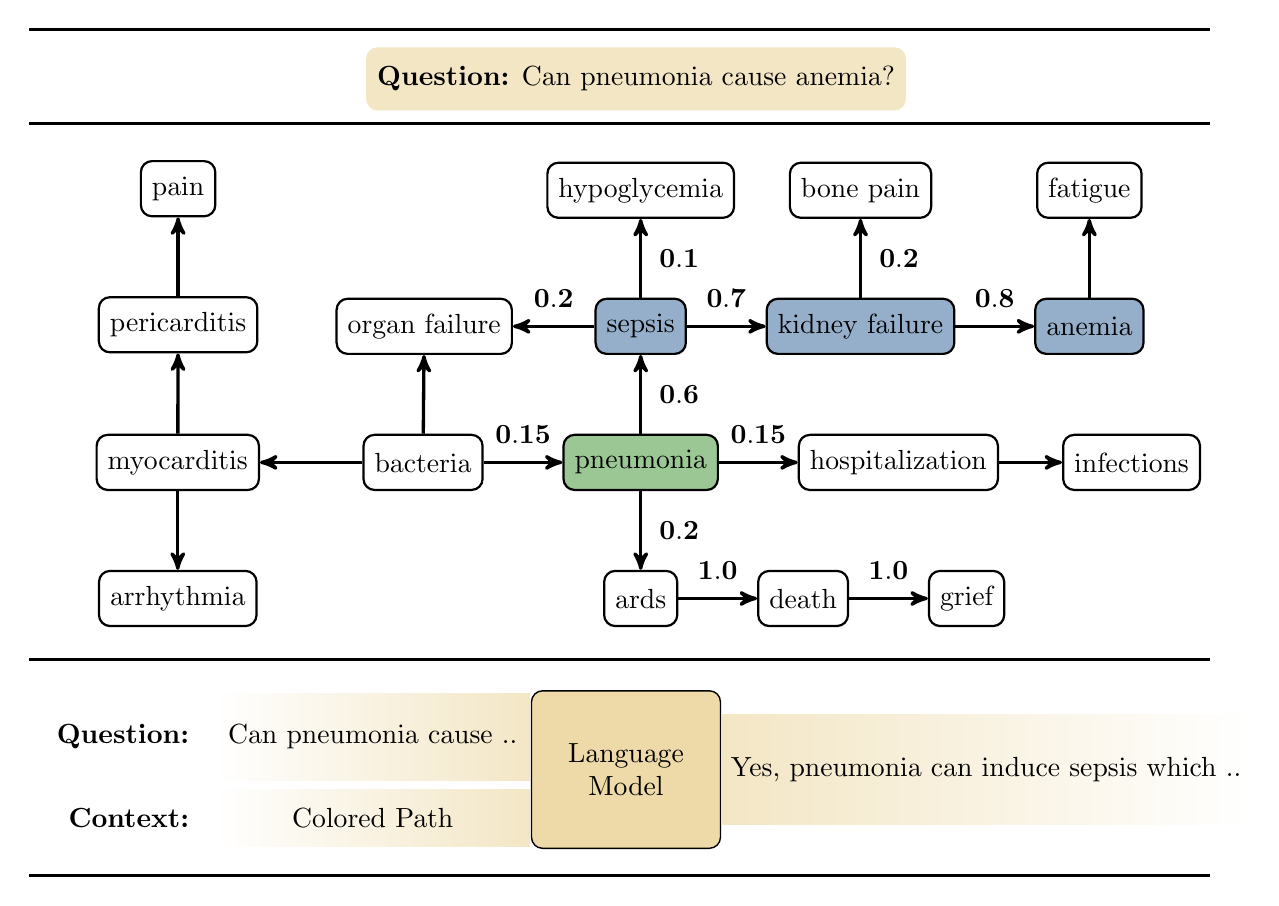
\begin{tikzpicture}
        %\tikzstyle{vertex}=[draw, rectangle, rounded corners, minimum width=1.8cm, minimum height=1.4cm, line width=0.8pt]
        \tikzstyle{vertex}=[draw, rounded corners, line width=0.8pt, inner sep=4pt, minimum height = 0.7cm]
        \tikzstyle{box}=[minimum height=0.8cm, minimum width = 6cm, inner sep=4pt, rounded corners]
        \tikzstyle{arrow} = [->, thick,>=stealth']
        
        
        %\node[draw, line width=1pt] (Corner) {};
        \node[vertex] (N1) {bacteria};
        \node[vertex, left = 1.3cm of N1] (myocarditis) {myocarditis};
        \node[vertex, below = 1cm of myocarditis] (arrhythmia) {arrhythmia};
        \node[vertex, above left = 1.02cm and 1.32cm of N1] (pericarditis) {pericarditis};
        \node[vertex, above = 1cm of pericarditis] (pain) {pain};
        \node[vertex, right = 1cm of N1, fill=tab20darkgreen!60] (pneumonia) {pneumonia};
        \node[vertex, right = 1cm of pneumonia] (hospitalization) {hospitalization};
        \node[vertex, right = 0.8cm of hospitalization] (infections) {infections};
        \node[vertex, above = 1cm  of pneumonia, fill=tab20darkblue!60] (sepsis) {sepsis};
        \node[vertex, above = 1cm of sepsis] (hypoglycemia) {hypoglycemia};
        \node[vertex, left = 1.035cm of sepsis] (organ) {organ failure};
        \node[vertex, below = 1cm of pneumonia] (ards) {ards};
        \node[vertex, right = 1cm of ards] (death) {death};
        \node[vertex, right = 1cm of death] (grief) {grief};
        
        \node[vertex, right = 1cm  of sepsis, fill=tab20darkblue!60] (kidney) {kidney failure};
        \node[vertex, above = 1cm  of kidney] (bone) {bone pain};
        \node[vertex, right = 1cm  of kidney, fill=tab20darkblue!60] (anemia) {anemia};
        \node[vertex, above = 1cm  of anemia] (fatigue) {fatigue};
        
         \node[draw, rounded corners, line width=0.5pt, inner sep=4pt,below left = 0.8cm and -1.5cm of ards, fill=brass!60, minimum height=2cm, minimum width = 2.4cm, align=center] (LM) {Language \\ Model};
         
        \node[box, fill=brass!40, label=left:{}, above right = 4.1cm and -1.5cm of N1] (MCQ)  {\textbf{Question:} Can pneumonia cause anemia?};
         
         \node[left color=white, right color=brass!40, above left = -1.15cm and 0cm of LM, fill=brass!40, minimum height=1.1cm, minimum width = 4cm, align=center] (q1) {Can pneumonia cause ..};
         \node[left color=white, right color=brass!40, below = 0.1cm of q1, fill=brass!40, minimum height=0.73cm, minimum width = 4cm, align=center] (q2) {Colored Path};
         \node[left = 0.2cm of q1, fill=white, minimum height=1.1cm, minimum width = 1.5cm, align=center] (t1) {\textbf{Question:}};
         \node[left = 0.2cm of q2, fill=white, minimum height=1.1cm, minimum width = 1.5cm, align=center] (t2) {\textbf{Context:}};
         \node[right color=white, left color=brass!40, right = 0cm of LM, fill=brass!40, minimum height=1.4cm, minimum width = 4cm, align=center] (q3) {Yes, pneumonia can induce sepsis which ..};

        
        %\node[above left = 0.3cm and -0.4cm of pericarditis] (a) {\textbf{a)}};
        %\node[above left = 0.2cm and -0.5cm of MCQ] (b) {\textbf{b)}};
        %\node[below left = 0.35cm and 3.4cm of ards] (c) {\textbf{c)}};

        %\node[left = 0.1cm of sepsis] (ps) {\textbf{0.7}};
        %\node[above = 0.1cm of pneumonia] (pf) {\textbf{0.1}};
        %\node[left = 0.1cm of ards] (pa) {\textbf{0.2}};
        %\node[above = 0.1cm of death] (pa) {\textbf{1.0}};
        %\node[above = 0.1cm of kidney] (ph) {\textbf{1.0}};
        
        \draw[arrow, line width=1.2pt] (N1) -- (myocarditis);
        \draw[arrow, line width=1.2pt] (N1) -- (organ);
        \draw[arrow, line width=1.2pt] (pneumonia) to node[right=0.1cm, pos=0.5]  {$\mathbf{0.6}$} (sepsis);
        \draw[arrow, line width=1.2pt] (pneumonia)  to node[right=0.1cm, pos=0.5]  {$\mathbf{0.2}$}(ards);
        \draw[arrow, line width=1.2pt] (pneumonia) to node[above=0.1cm, pos=0.5]  {$\mathbf{0.15}$} (hospitalization);
        \draw[arrow, line width=1.2pt] (N1) to node[above=0.1cm, pos=0.5]  {$\mathbf{0.15}$} (pneumonia);
        \draw[arrow, line width=1.2pt] (kidney) to node[above=0.1cm, pos=0.5]  {$\mathbf{0.8}$} (anemia);
        \draw[arrow, line width=1.2pt] (kidney) to node[right=0.1cm, pos=0.5]  {$\mathbf{0.2}$} (bone);
        \draw[arrow, line width=1.2pt] (anemia) -- (fatigue);
        \draw[arrow, line width=1.2pt] (hospitalization) -- (infections);
        \draw[arrow, line width=1.2pt] (sepsis) to node[right=0.1cm, pos=0.5]  {$\mathbf{0.1}$} (hypoglycemia);
        \draw[arrow, line width=1.2pt] (sepsis) to node[above=0.1cm, pos=0.5]  {$\mathbf{0.2}$} (organ);
        \draw[arrow, line width=1.2pt] (myocarditis) -- (pericarditis);
        \draw[arrow, line width=1.2pt] (myocarditis) -- (arrhythmia);
        \draw[arrow, line width=1.2pt] (pericarditis) -- (pain);
        
        \draw[arrow, line width=1.2pt] (sepsis) to node[above=0.1cm, pos=0.5]  {$\mathbf{0.7}$} (kidney);
        \draw[arrow, line width=1.2pt] (ards) to  node[above=0.1cm, pos=0.5]  {$\mathbf{1.0}$} (death);
        \draw[arrow, line width=1.2pt] (death) to  node[above=0.1cm, pos=0.5]  {$\mathbf{1.0}$} (grief);

        \draw [draw, line width=1.2pt] (-5,5.5) -- (10,5.5);
        \draw [draw, line width=1.2pt] (-5,4.3) -- (10,4.3);
        \draw [draw, line width=1.2pt] (-5,-2.5) -- (10,-2.5);
        \draw [draw, line width=1.2pt] (-5,-5.25) -- (10,-5.25);
        %\draw[thick,rounded corners]     ($(inflammation.north west)+(-0.2,0.89)$) rectangle ($(death.south east)+(0.5,-0.3)$);
        
        %\draw[thick,rounded corners]     ($(ards.south west)+(-4,-0.3)$) rectangle ($(C.south east)+(0.5,-3)$);
    \end{tikzpicture}
    \caption{An excerpt from CauseNet~\cite{Heindorf2020Causenet} showing the entity \textit{pneumonia} together with its neighborhood containing causes and effects. 
            Each edge depicts a \textit{cause} relation. Given the question \textit{``Can pneumonia cause anemia?''}, the search
            starts at the entity \textit{pneumonia}. Following the path \textit{(pneumonia, sepsis, kidney failure, anemia)}, the question 
            can be answered with ``yes''. The numbers on the edges show the probability of taking this edge under the current 
            policy $\pi_{\theta}(a_t | s_t)$. For brevity, we only show the relevant probabilities for the given path. The lower part of the figure shows the possibility to combine our agent with a language model. In that setup, we provide the paths the agent learned for a question as additional context 
            to the language model. We briefly explore this setup in Section~\ref{sec:evaluation-approach}.
            }
    \label{fig:graph_example}
\end{figure}

\section{Network Architecture}
\label{sec:network}
 We use a Long Short-Term Memory (LSTM)~\cite{Hochreiter1997LSTM} to parametrize our agent. LSTMs were introduced to improve 
 standard RNNs and can better handle the vanishing gradient problem~\cite{Hochreiter1997LSTM}. 
 Additionally, we experimented with a simple feedforward architecture 
 but found that incorporating the path history is crucial for our needs.
 This aligns with previous research, where approaches such as MINERVA~\cite{Das2018Minerva} and SRN~\cite{Qiu2020Stepwise} 
 also used LSTMs and GRUs. Just CONQUER~\cite{Kaiser2021Reinforcement} used a feedforward architecture, but they only 
 considered paths of length one.


 Let $\mathbf{q} \in \mathcal{R}^d$ be the embedding of the question $q$ and $\mathbf{E} \in \mathcal{R}^{|\mathcal{E}| \times d}$ the 
 embedding matrix containing the embeddings for each entity $e \in \mathcal{E}$ of the knowledge graph.
 The parameter $d$ specifies the dimension of the embeddings.
  $\mathcal{K}$. The LSTM formula is then applied as follows:

\begin{equation}
	\mathbf{h_t}=
    \begin{cases}
      LSTM(\mathbf{0}; [\mathbf{q}, \mathbf{e_c}]), & \text{if}\ t=0 \\
      LSTM(\mathbf{h_{t-1}}, [\mathbf{q}; \mathbf{e_t}]), & \text{otherwise}
    \end{cases}
\end{equation}

where $\mathbf{h_t} \in \mathcal{R}^{2d}$ represents the hidden state vector (history) of the LSTM, 
and $[;]$ is the vector concatenation operator. At each time step, the LSTM takes the previous history
 $\mathbf{h_{t-1}}$ and the concatenation of the question embedding $\mathbf{q}$ and the current node embedding
 $\mathbf{e_t} \in \mathcal{R}^{d}$ to produce $\mathbf{h_t}$. In the first time step, $\mathbf{h_0}$ is initialized with the
 zero vector and $\mathbf{e_0} = \mathbf{e_c}$, where $\mathbf{e_c}$ is the embedding of the entity corresponding to 
 the cause found in the current question. 
 %Previous approaches like MINERVA~\cite{Das2018Minerva} also 
 %concatenated the previous action embedding $\mathbf{a_{t-1}}$ to $\mathbf{e_t}$. However, 
 %we found this not to be necessary. Generally, it should be implicitly included through the
 %history $\mathbf{h_t}$.

 On top of the LSTM, we stack two feedforward networks: one for the policy 
 network $\pi_\theta(a_t | s_t)$ and one for the value network $V_\psi(s_t)$.
 In Section ~\ref{sec:env}, we defined the action space $\mathcal{A}(s_t)$ at time step $t$ and state $s_t = (\mathbf{q}, e_t, \mathbf{e_t}, \mathbf{h_t}, e_e)$
  to contain all neighbors of the entity $e_t$.
  Therefore, we introduce an embedding matrix $\mathbf{A_t} \in \mathcal{R}^{|A(s_t)| \times 2d}$, where
  the rows contain the embeddings of the actions  $a_t \in \mathcal{A}(s_t)$. Consequently, 
  the output of the policy network $\pi_{\theta}(a_t|s_t)$ is computed as follows:
\begin{equation}
	\begin{split}
	\pi_\theta(a_t | s_t) = \sigma(\mathbf{A_t} \times W_2 \times ReLU(W_1 \times \mathbf{h_t})) \\
	a_t \sim Categorical(\pi_\theta(a_t | s_t))
	\end{split}
\end{equation}

where $W_1 \in \mathcal{R}^{h \times 2d}$ and $W_2 \in \mathcal{R}^{2d \times h}$ are weight matrices with hidden dimension $h$ and $\sigma$ is the softmax operator.
The final output of the policy network is a categorical probability distribution over 
all actions $a_t \in \mathcal{A}(s_t)$.
Similarly, the output of the value network $V_{\psi}(s_t)$ is computed with the 
following feedforward network:
\begin{equation}
	V_{\psi}(s_t) = W_4 \times ReLU(W_3 \times \mathbf{h_t})
\end{equation}
where $W_3\in \mathcal{R}^{h \times 2d}$ and $W_4\in \mathcal{R}^{1 \times h}$ are weight matrices with hidden dimension $h$, and the output is a scalar that
estimates the future reward from state $s_t$ onwards. Overall, the weights of
the LSTM are shared between the policy and value network, while each network 
has its own weights in the form of its feedforward head.


\section{Training of the Reinforcement Learning Agent}
\label{sec:approach-description}

In the following, we describe the training procedure of our reinforcement learning agent.
This includes the pre-processing of the questions, the sampling of path rollouts, and the update rules 
for the weights of the agent.
We start with the observation that CauseNet~\cite{Heindorf2020Causenet} does not contain 
negative information. Thus, we only train the agent on positive causal questions, i.e., questions 
whose answer is ``yes''. 
Similarly, we must remove all questions where the cause, effect, or both cannot be found in CauseNet. 
In that case, we are restricted by CauseNet, so there is nothing to learn.

%Training the agent on both, positive and negative questions, would result in 
%conflicting reward signals. For positive questions we would give the agent a reward of 
%one if a path is found and when given a negative question we would have to give a 
%reward of one when no path is found.

Algorithm~\ref{alg:algorithm} displays the pseudocode of the whole training phase.
The pseudocode assumes that only positive causal questions, where cause and effect can be found in 
CauseNet, remain in the given $questions$.
First, we pre-process the questions by linking the cause and effect to the corresponding 
entities $e_c$ and $e_e$ in CauseNet. This is followed by the computation of embeddings for the question and entities.\footnote{We use GloVe~\cite{Pennington2014Glove} embeddings to embed the questions and entities. For more details, see Section~\ref{sec:impl-details}}
Next, the weights $\theta$ and $\psi$ of the agent are initialized. 
In the default setup, both are initialized randomly.
In the case of a preceding supervised learning phase (Section~\ref{sec:supervised}), the weights 
of the policy network $\theta$ are initialized with the resulting weights from the supervised learning.

Afterward, we start sampling path rollouts from the environment via the current policy network
$\pi_\theta(a_t | s_t)$. Each path rollout has the same length $T$. Hence, the agent 
should learn to use the \textit{STAY} action in case it arrives at 
the target entity before a length of $T$ is reached. Given a pre-processed question $q$, we construct the first state $s_0$.
Subsequently, the agent interacts with the environment for $T$ time steps. At each time step, 
the agent applies an action $a_t$ and receives a reward $r_t$ while the environment evolves 
via the transition function $\delta(s_t, a_t)$ to the next state $s_{t+1}$.
This procedure is continued until a full batch of path rollouts is accumulated.


The training of the agent is facilitated via the Synchronous Advantage Actor-Critic (A2C)~\cite{Mnih2016A2C} algorithm, 
as described in Section~\ref{subsec:rl}. The policy network 
$\pi_\theta(a_t | s_t)$ takes the role of the actor while the value network $V_\theta(s_t)$ takes 
the role of the critic. We briefly experimented with Proximal Policy Optimization (PPO)~\cite{Schulman2017PPO} but found no significant performance improvements.

Thus, the update rule for the policy network $\pi_\theta(a_t | s_t)$ looks as follows:
\begin{equation}
  \nabla_{\theta} J(\theta) = - \frac{1}{B} \sum_{i}^{B} \sum_{t=0}^{T-2} \nabla_{\theta} \log(\pi_{\theta} (a_t | s_t)) \, \mathcal{A}_{t}^{\psi}
\end{equation}
where $B$ is the batch size, T the path rollout length, and $\mathcal{A}_{t}^{\psi}$
the generalized advantage estimate (GAE) as described in Section~\ref{subsec:rl}.

As commonly done, we add an entropy regularization term to the objective~\cite{Das2018Minerva, Kaiser2021Reinforcement}.
The entropy regularization should help the agent with the exploitation vs. exploration tradeoff.
Specifically, it should encourage exploration during training and stop the agent from getting 
stuck in local minima. Therefore, the resulting policy should be more robust and have a higher diversity
 of explored actions. We compute the average entropy of the action distribution of
 $\pi_{\theta}(a_t | s_t)$ over all actions $a_t \in \mathcal{A}(s_t)$ at each time step $t$ and take the average over the 
 whole batch:
\begin{equation}
	H_{\pi_\theta} = \frac{1}{B(T-1)} \sum_{i}^{B} \sum_{t=0}^{T-2} (- \hspace{-0.3cm}\sum_{a_t \in \mathcal{A}(s_t)} \pi_\theta(a_t | s_t)  \log \pi_\theta(a_t | s_t))
\end{equation}

The final update for the policy network becomes:
\begin{equation}
  \theta = \theta - lr \cdot(\nabla_{\theta} J(\theta) + \beta H_{\pi_\theta})
\end{equation}
where $lr$ is the learning rate and $\beta$ is a hyperparameter 
that determines the weight of the entropy regularization term.

Simultaneously, we update the value network $V_{\psi}(s_t)$ via the mean-squared error between 
the $\lambda$-return and the predictions of the value network:
\begin{equation}
		\nabla_{\psi} J(\psi)= \frac{1}{B (T-1)} \sum_{i}^{B} \sum_{t=0}^{T-2} \nabla_{\psi} (R_t(\lambda) - V_{\psi}(s_t))^2
\end{equation}
where $R_t(\lambda)$ is the $\lambda$-return as described in Section~\ref{subsec:rl}.
Therefore, the final update for the value network becomes:
\begin{equation}
  \psi = \psi - lr \cdot \nabla_{\psi} J(\psi)
\end{equation}
where $lr$ is the learning rate. In our experiments, we use the same learning rate
$lr$ for both networks. This is not compulsory and they could also use 
different learning rates. Overall, the training loop of selecting path rollouts and 
using them to update the policy and value networks is repeated for a number of 
optimization $steps$.

\begin{algorithm}
	\DontPrintSemicolon
	\caption{Pseudocode of the training procedure for the policy 
	network $\pi_{\theta}(a_t | s_t)$ and value network $V_\psi(s_t)$ 
	as described in Section~\ref{sec:approach-description}.}%
	\label{alg:algorithm}%
	\textbf{Input:} Knowledge graph $\mathcal{K}$, questions $questions$, 
	optimization steps $steps$, batch size $B$, path rollout length $T$, learning rate $lr$,
	entropy weight $\beta$, discount factor $\gamma$, GAE lambda $\lambda$  \\
	\textbf{Output:} Trained Agent $\theta$, $\psi$ \\
	\SetKwFunction{F}{TrainAgent}
	\SetKwProg{Fn}{Function}{:}{\KwRet $\theta$}
	\Fn{\F{$\mathcal{K}$, $questions$, $steps$, $B$, $T$, $lr$, $\beta$, $\gamma$, $\lambda$}}{%
		$processed\_questions = [ \ ]$\;
		\For{\textbf{each} $q$ \textbf{in} $questions$}{%
			Link the cause and effect of $q$ to entities $e_c$ and $e_e$ in $\mathcal{K}$\;
			Compute embeddings $\mathbf{q}$, $\mathbf{e_c}$ for $q$, $e_c$\;
			$processed\_questions.append((\mathbf{q}, e_c, \mathbf{e_c}, e_e))$
		}
		\;
		Initialize agent weights $\theta$, $\psi$\;
		$path\_rollouts = [\,]$\;
		$step = 0$\;
		\While{step < steps}{%
			$path\_rollout = [\,]$\;
			$(\mathbf{q}, e_c, \mathbf{e_c}, e_e) = SampleUniform(processed\_questions)$\;
			$s_0 = (\mathbf{q}, e_c, \mathbf{e_c}, \mathbf{0}, e_e)$\; \label{ln:17}
			\For{$t = 0$ \textbf{to} $T-1$}{%
				$a_t = SampleCategorical(\pi_{\theta}(a_t | s_t))$\;
				Receive state $s_{t+1} = \delta (s_t, a_t)$ and reward $r_t = \mathcal{R}(s_{t+1})$\; \label{ln:20}
				$path\_rollout.append((s_t, a_t, r_t))$\;
			}
			$path\_rollouts.append(path\_rollout)$\;
			\;
			\If{$|path\_rollouts| = B$}{%
				Compute the GAE $\mathcal{A}_t^{\psi}$ and $\lambda$-returns $R_t(\lambda)$ for each episode in $path\_rollouts$ using $\lambda, \gamma$ \;
				$policy\_update, \ value\_update = 0$\;
				\For{\textbf{each} $((s_0, a_0, r_0, \mathcal{A}_0^{\psi}, R_0(\lambda)),\dots, (s_{T-2}, a_{T-2}, r_{T-2}, \mathcal{A}_{T-2}^{\psi}, R_{T-2}(\lambda)))$ \textbf{in} path\_rollouts}{%
					$policy\_update \mathrel{+} = \sum_{t=0}^{T-2} \nabla_{\theta} \log \pi_{\theta}(a_t | s_t) \ \mathcal{A}_t^{\psi}$\;
					$value\_update \mathrel{+} = \sum_{t=0}^{T-2} \nabla_{\psi} (R_t(\lambda) - V_{\psi}(s_t))^2$\;
				}
				Compute the entropy regularization term $H_{\pi_{\theta}}$\;
				$policy\_update = - \frac{policy\_update}{|path\_rollouts|}$, $\ value\_update = \frac{value\_update}{|path\_rollouts| \cdot (T-1)}$\;
				$\theta = \theta - lr \cdot (policy\_update + \beta H_{\pi_{\theta}})$\;
				$\psi = \psi - lr \cdot value\_update$\;
				$path\_rollouts = [\,]$\;
				$step = step + 1$\;
			}
		}
	}
\end{algorithm}

\section{Search Strategy}
\label{sec:search}
At inference time, the agent receives both positive and negative questions.
To answer a given question, we sample multiple paths $p$ of length $T$ from the agent. 
If any path contains the entity $e_e$, the agents answers the question with ``yes'' and ``no'' otherwise.
In case the cause, effect, or both cannot be found in CauseNet, the question 
is answered with ``no'' per default.

For each path rollout $((s_0, a_0),(s_1, a_1), \dots, (s_{T-2}, a_{T-2}))$, the
path that was taken on the graph consists of the entity $e_0$ in $s_0$ and 
the actions taken at each time step $t$, i.e., $p = (e_0, e_1,\dots, e_{T-1})$ where $a_{t-1} = e_t \in \mathcal{E}$ for $t > 0$.

The probability of path $p$ can be formulated as follows:
 \begin{equation}
\mathbb{P}(p) = \prod_{t=0}^{T-2} \pi_{\theta}(a_t |s_t)
\label{eq:decoding}   
 \end{equation}

 where the probability of $p$ is computed as the product of the probabilities of taking action $a_t$ at state $s_t$ under the current policy $\pi_{\theta}(a_t | s_t)$ for $t \in \{0,\dots,T-2\}$.
 Note that, this formulation has a similar autoregressive nature as a language model objective~\cite{Bengio2003LM}. 
The next action $a_t$ depends on the current state $s_t$ and implicitly, through the history $\mathbf{h_t}$, on all previous states.
 Thus, we use decoding methods from
  the language model literature to sample paths from the agent. Specifically,
we consider greedy decoding and beam search, as done by prior works~\cite{Das2018Minerva, Qiu2020Stepwise}.

%Further decoding methods like 
%Top-K~\cite{Fan2018TopK} or Nucleus Sampling~\cite{Holtzman2020Nucleus}
% are not applicable because we are not 
%optimizing for diversity but instead want to find the most probable paths.\todo{Verify this in
%experiments or rewrite?}

In the following, we illustrate the decoding methods on the basis of the example 
in Figure~\ref{fig:graph_example}. The figure shows an excerpt from CauseNet, and each edge 
is annotated with the probability of taking this edge under the current policy.
Given the question \textit{``Can pneumonia cause anemia?''} the search starts at the 
entity \textit{pneumonia}.

Greedy decoding takes the action with the highest probability at each time step, i.e.,
$arg\,max_{a_t \in \mathcal{A}(s_t)} \ \pi_{\theta}(a_t | s_t)$. So in the example,
 the agent would select \textit{sepsis} in the first time step, \textit{kidney failure} in
 the second time step, and \textit{anemia} in the third time step. 
 However, one disadvantage of greedy decoding is its myopic
  behavior. Therefore, greedy decoding might miss high-probability actions in later
  time steps. Beam search tries to alleviate this problem by always keeping a set of the 
  best partial solutions up to the current timestep. The size of this set is a hyperparameter called \textit{beam width}.
  In our case, partial solutions are paths of length $t$, where $t$ is the 
  current timestep. Furthermore, the paths are ranked by their probability, as defined in
  Equation~\ref{eq:decoding}.
   
  Assuming a beam width of two, we demonstrate the decoding for the example in Figure~\ref{fig:graph_example}. At each time step, we show
  the two top paths together with their probability:
  \par\noindent\rule{\textwidth}{0.4pt}
  \begin{itemize}
		\item \textbf{Time Step 1}
				%\textbf{Partial Solutions:} 
        \begin{itemize}
          \item \textbf{Path 1:} \textit{(pneumonia, sepsis)} $\rightarrow$ $0.6$
          \item	\textbf{Path 2:} \textit{(pneumonia, ards)} $\rightarrow$ $0.2$
        \end{itemize}
	\end{itemize}
  \par\noindent\rule{\textwidth}{0.4pt}
  \begin{itemize}
		\item \textbf{Time Step 2}
        \begin{itemize}
          \item	\textbf{Path 1:} \textit{(pneumonia, sepsis, kidney failure)} $\rightarrow$ $0.6 \cdot 0.7 = 0.42$
          \item	\textbf{Path 2:} \textit{(pneumonia, ards, death)} $\rightarrow$ $0.2 \cdot 1.0 = 0.2$
        \end{itemize}
	\end{itemize}
  \par\noindent\rule{\textwidth}{0.4pt}
  \begin{itemize}
		\item \textbf{Time Step 3}
        \begin{itemize}
          \item	\textbf{Path 1:} \textit{(pneumonia, sepsis, kidney failure, anemia)} $\rightarrow$ $0.42 \cdot 0.8 = 0.336$
          \item	\textbf{Path 2:} \textit{(pneumonia, ards, death, grief)} $\rightarrow$ $0.2 \cdot 1.0 = 0.2$
        \end{itemize}
	\end{itemize}
  \par\noindent\rule{\textwidth}{0.4pt}

  Finally, the agent checks whether one of the two paths found by beam search contains the 
  effect. If that is the case, the agent answers the question with ``yes'' and ``no'' otherwise.
In this example, \textit{anemia} is found, so the agent answers with ``yes''.
In practice, the computations are done in log space to avoid numerical problems.

In our case, beam search can be viewed as an interpolation between greedy decoding and breadth-first search (BFS).
As the beam width increases, the search strategy of the agent gets closer to an exhaustive search.
This should increase performance but might make the task too easy if the beam width is set too high.
However, at the same time, there are also runtime considerations. While a higher beam width increases performance, it will also increase the runtime.
We further analyze these trade-offs in Sections~\ref{sec:decoding-analysis} and~\ref{sec:inference time}.

\section{Bootstrapping via Supervised Learning}
\label{sec:supervised}

Reinforcement learning algorithms often take a long time to converge due to their
trial-and-error nature combined with large action spaces and sparse rewards~\cite{Xiong2017DeePpath, Lin2020RewardShaping}.
Thus, the reinforcement learning agent can be bootstrapped, by first training
it on a series of expert demonstrations. For example, AlphaGo~\cite{Silver2016AlphaGO} trained 
the agent on demonstrations from expert Go players before continuing with their reinforcement learning
algorithm.

In our case, the expert demonstrations come from a breadth-first search (BFS)
on CauseNet. This setup was first explored by DeepPath~\cite{Xiong2017DeePpath}.
Subsequent approaches like MINERVA~\cite{Das2018Minerva} and SRN~\cite{Qiu2020Stepwise} discarded
supervised learning in favor of several improvements. These improvements included the introduction 
of an LSTM in the policy network~\cite{Das2018Minerva} or the usage of attention mechanisms~\cite{Qiu2020Stepwise}.
Despite that, we decided to reintroduce supervised learning
due to the lack of relation types and the resulting large action space in CauseNet.
The original DeepPath~\cite{Xiong2017DeePpath} implementation used a two-sided randomized BFS.
Given entities $e_1$ and $e_2$, DeepPath selects a random node $e_r$. Next, DeepPath runs a 
BFS between $e_1 \rightarrow$ $e_r$ and $e_r \rightarrow$ $e_2$ and concatenates the found paths. This setup is supposed 
to help the agent to learn longer paths and not be biased toward shorter ones. However, in a pilot study, we found it unnecessary 
and used a standard BFS directly between $e_1$ and $e_2$.

\begin{algorithm}
	\DontPrintSemicolon
	\caption{The supervised learning algorithm that is used to 
	bootstrap our agent. In the first step, we use a BFS to create expert demonstrations 
	from the training questions. Afterward, we train the policy network $\pi_{\theta}(a_t | s_t)$
	via the standard REINFORCE update using the expert demonstrations.
	}%
	\label{alg:supervised-alg}%
	\textbf{Input:} Knowledge graph $\mathcal{K}$, questions $questions$, 
	optimization steps $steps$, batch size $B$, path rollout length $T$, learning rate $lr$,
	supervised ratio $\alpha$, entropy weight $\beta$ \\
	\textbf{Output:} Trained Agent $\theta$ \\
	\SetKwFunction{F}{SupervisedTrainAgent}
	\SetKwProg{Fn}{Function}{:}{\KwRet $\theta$}
	\Fn{\F{$\mathcal{K}$, $questions$, $steps$, $B$, $T$, $lr$, $\alpha$, $\beta$}}{%
		Sample $\lfloor \alpha \cdot |questions| \rfloor$ $\overline{Q}$ from $questions$\;
		$path\_rollouts = [ \ ]$\;
		\For{\textbf{each} $q$ \textbf{in} $\overline{Q}$}{%
			Link the cause and effect of $q$ to entities $e_c$ and $e_e$ in $\mathcal{K}$\;
			%$((s_0, a_0),\dots, (s_{T-2}, a_{T-2}))  = $ \texttt{BFS($\mathcal{K}, q, c, e, T$)} \;
			\tcp*[l]{Run BFS, note that $e_0=e_c$ and $e_n=e_e$}
			$(e_0, e_1, \dots, e_n) = $ \texttt{BFS($\mathcal{K}, e_c, e_e, T$)}\;
			Compute embeddings $\mathbf{q}$ and $\mathbf{e_t}$ for question $q$ and $0 \leq t \leq n-1$\;
			Build $path\_rollout$ $((s_0, a_0, r_0),\dots, (s_{n-1}, a_{n-1}, r_{n-1}))$ \newline
			\hspace*{0.3cm} where $s_t=(\mathbf{q}, e_t, \mathbf{e_t}, \mathbf{0}, e_e)$, $a_t=e_{t+1}$, and $r_t=1$ with $0 \leq t \leq n-1$\;
			\If{$n-1 < T-2$}{
				Pad the $path\_rollout$ with $(s_t, a_t, r_t)$ where $s_t=(\mathbf{q}, e_{n-1}, \mathbf{e_{n-1}}, \mathbf{0}, e_e)$, 
				\hspace*{0.3cm} $a_t = \textit{STAY}$, and $r_t = 1$ for $n-1 < t \leq T-2$\;
			}
			$path\_rollouts.append(((s_0, a_0, r_0),\dots, (s_{T-2}, a_{T-2}, r_{T-2})))$\;
		}
		$batches = \texttt{BuildBatches}(path\_rollouts, B)$\;
		\;
		Initialize agent weights $\theta$\;
		\For{step $=$ 0 \textbf{to} $steps - 1$}{%
			$batch = batches[step \ \% \ |batches|]$\;
			$policy\_update = 0$\;
			\For{$\textbf{each}((s_0, a_0, r_0),\dots, (s_{T-2}, a_{T-2}, r_{T-2}))$ \textbf{in} batch}{%
				$policy\_update \mathrel{+} = \sum_{t=0}^{T-2} \nabla_{\theta} \log \pi_{\theta}(a_t | s_t) \, r_t$\;
			}
			Compute the entropy regularization term $H_{\pi_{\theta}}$\;
			$policy\_update = - \frac{policy\_update}{|batch|}$\;
			$\theta = \theta - lr \cdot (policy\_update + \beta H_{\pi_{\theta}})$\;
		}
	}
\end{algorithm}
Algorithm~\ref{alg:supervised-alg} shows the supervised training procedure.
First, we randomly select a subset $\overline{Q}$ of size $\alpha \cdot |questions|$
 of the training questions, where $\alpha$ is a hyperparameter.
Subsequently, we run a BFS on the cause $e_c$ and effect $e_e$ of each question in $\overline{Q}$
and build a path rollout for each found path. If a path rollout is shorter than
the path rollout length $T$, it is padded with the \textit{STAY} action.\footnote{For simplicity, the pseudocode assumes that a path of length less than or equal to $T$ can 
			 be found between $e_c$ and $e_e$ for each question $q$. In practice, the question $q$
			 would have to be discarded if no path is found.} Next, we 
update the policy network $\pi_{\theta}(a_t | s_t)$ via the standard REINFORCE update as described
in Section~\ref{subsec:rl}:
\begin{equation}
  \nabla_{\theta} J(\theta) = - \frac{1}{B} \sum_{i}^{B} \sum_{t=0}^{T-2} \nabla_{\theta} \log(\pi_{\theta} (a_t | s_t)) \, r_t + \beta H_{\pi_\theta}
\end{equation}
where $B$ is the batch size, $T$ the path rollout length, and $H_{\pi_\theta}$ the entropy regularization from Section~\ref{sec:approach-description}. 
During supervised training, the reward $r_t$ is set to $1$ at each step.
Note that we only train the policy network $\pi_{\theta}(a_t | s_t)$ during supervised 
learning. We excluded the value network because we do not have negative examples in the current setup and found the current 
setup to work well enough.
Afterward, we further train the policy value networks via Algorithm~\ref{alg:algorithm}, as explained in Section~\ref{sec:approach-description}.


\section{Reward Shaping}
\label{sec:reward-shaping}

Under the current setup, the agent only receives a reward at the final time step $T-1$ if it 
finds the target entity, such that $e_{T-1} = e_e$.
Thus, in large action spaces, the agent might not receive any 
learning signal for a long time if it only rarely finds correct paths. 
To mitigate this problem, we introduced a supervised learning 
procedure in the previous section that provides a series of expert demonstrations to the agent.
In the following, we explore a different direction by introducing auxiliary reward signals through a 
reward shaping technique.

Prior works for reinforcement learning on knowledge graphs already experimented with reward shaping techniques: (1) Lin et al.~\cite{Lin2020RewardShaping} scored 
the last node with a knowledge graph embedding model if the path was not correct, (2) Qiu et al.~\cite{Qiu2020Stepwise} scored each 
path by its cosine similarity with the question. Conversely, we experiment with a 
different technique introduced by Yasunaga et al.~\cite{Yasunaga2021QAGNN} for their QA-GNN model.
Yasunaga et al. use a language model to score the entities on a knowledge graph according to their relevance 
to the question. Specifically, the score should represent how semantically close an entity is to the question. This is particularly suitable in our case because the entities in CauseNet also 
have labels in natural language.

Consequently, we adapt this approach to our task by scoring the last entity $e_{T-1}$ on paths that were not successful.
The idea is that the agent should still receive some indication of how ``good'' a path is if it does 
not lead to the target entity. 
Therefore, given a question $q$ and entity $e_{T-1}$ the score function is defined 
as follows~\cite{Yasunaga2021QAGNN}:
\begin{equation}
  Score(q, e_{T-1}) = LM_{head}(LM_{enc}([q;e_{T-1}]))
\end{equation}
where $LM_{enc}$ is the encoder of the language model, $LM_{head}$ is a two-layer feedforward network, and 
$[;]$ the concatenation operator.


The new reward function $\mathcal{R}'(s_{T-1})$ returns the default reward $\mathcal{R}(s_{T-1})$ if $e_{T-1}=e_e$
and $Score(q, e_{T-1})$ otherwise. Just like the default reward it is $0$ at all other time steps $t < T-1$.
We experimented with scoring each entity on a path with little success.
Hence, given state $s_{T-1}$ the new reward function is defined as~\cite{Lin2020RewardShaping}:
\begin{equation}
  \mathcal{R}'(s_{T-1}) = \mathcal{R}(s_{T-1}) + (1 -  \mathcal{R}(s_{T-1})) \cdot Score(q, e_{T-1}) \cdot \omega  
\end{equation}

where $\mathcal{R}(s_t)$ is the default reward defined in Section~\ref{sec:env} and 
$\omega$ is a hyperparameter. Generally, the scores of the language model are not on the same scale 
as the reward $\mathcal{R}(s_t)$. Thus, $\omega$ is used to determine the weight of the score 
and scale it appropriately so that the auxiliary reward does not dominate over the default 
reward.

The addition of reward shaping only requires minor changes in the environment setup.
The states $s_t$ currently only contain the question embeddings $\mathbf{q}$. 
For the new reward function to receive the necessary information, we must 
add the question $q$ itself to each state, i.e., $s_t = (q, \mathbf{q}, e_t, \mathbf{e_t}, \mathbf{h_t}, e_e)$.
Additionally, we need to replace $\mathcal{R}(s_t)$ with $\mathcal{R}'(s_t)$ in Algorithm~\ref{alg:algorithm} Line~\ref{ln:20}.
Reward shaping is not used during supervised learning because supervised learning 
only uses correct paths.         % INCLUDE: approach
% !TEX root = proposal.tex
%
\chapter{Work Plan}
\label{sec:pan}


\begin{figure}[h]
\hspace*{-2cm}
\resizebox{1.2\linewidth}{!}{
\begin{ganttchart}[y unit title=0.5cm,
y unit chart=0.7cm,
vgrid={*{6}{draw=none},dotted},
hgrid,x unit=15mm,
hgrid style/.style={draw=black!10, line width=.9pt},
%title label anchor/.style={below=-1.6ex},
title/.style={fill=black!20, draw},
%title/.style={line width=1.8pt},
bar/.style={fill=tab20lightblue, draw},
milestone/.append style={xscale=3},
%title left shift=0,
%title right shift=0,
title height=1,
x unit=3pt,
progress label text={},
bar height=0.7,
group right shift=0,
group top shift=.6,
time slot format=simple,
group height=.3]{1}{154}
%labels
\gantttitle{July}{20} 
\gantttitle{Aug.}{31} 
\gantttitle{Sept.}{30} 
\gantttitle{Oct.}{31}
\gantttitle{Nov.}{30}
\gantttitle{Dec.}{12} \\
\gantttitlelist{1,...,22}{7}\\
%tasks
\ganttgroup{Literature Review}{2}{28} \\
\ganttbar{(Causal) QA}{2}{28} \\
\ganttbar{Policy Gradients}{2}{28} \\

\ganttgroup{Implementation}{5}{140} \\
\ganttbar{Setup CauseNet}{5}{21} \\
\ganttbar{Setup Datasets}{5}{21} \\
\ganttbar{Select Frameworks}{5}{35} \\
\ganttbar{Binary Questions}{8}{49} \\
\ganttbar{Cause/Effect Questions}{43}{84} \\
\ganttbar{Complex Questions}{71}{140} \\

\ganttgroup{Experiments}{50}{147} \\
\ganttbar{Comparison Baselines}{50}{147} \\
\ganttbar{Ablation Study}{78}{147} \\

\ganttgroup{Thesis Writing}{2}{153} \\
\ganttbar{Introduction}{2}{21} \\
\ganttbar{Related Work}{2}{42} \\
\ganttbar{Approach}{22}{140} \\
\ganttbar{Implementation}{43}{140} \\
\ganttbar{Evaluation}{71}{147} \\
\ganttbar{Discussion}{113}{153} \\
\ganttbar{Conclusion}{113}{153} \\ \\

\ganttmilestone{Binary Questions}{49} \\
\ganttmilestone{Cause/Effect Questions}{84} \\
\ganttmilestone{Thesis Draft}{140} \\
\ganttmilestone{Complex Questions}{140} \\
\ganttmilestone{Submission}{153}
%relations 
%\ganttlink{elem0}{elem1} 

\end{ganttchart}}
\caption{Work plan of the thesis.}
\end{figure}       % INCLUDE: plan
% !TEX root = proposal.tex
%
\renewcommand{\labelenumii}{\arabic{enumi}.\arabic{enumii}}
\renewcommand{\labelenumiii}{\arabic{enumi}.\arabic{enumii}.\arabic{enumiii}}
\renewcommand{\labelenumiv}{\arabic{enumi}.\arabic{enumii}.\arabic{enumiii}.\arabic{enumiv}}

\chapter{Thesis Structure}
\label{sec:structure}

\begin{enumerate}
    \item Introduction
    \item Related Work
    \begin{enumerate}
        \item Causal Question Answering
        \item Causal Knowledge Graphs
        \item Knowledge Graph Reasoning with Reinforcement Learning
    \end{enumerate}
    \item Approach
    \begin{enumerate}
        \item Preliminaries
        \begin{enumerate}
            \item CauseNet
            \item Reinforcement Learning
            \item Language Models
        \end{enumerate}
        \item Problem Definition -- Environment
        \item Approach Description
    \end{enumerate}
    \item Implementation
    \begin{enumerate}
        \item Project Structure
        \item Frameworks
    \end{enumerate}
    \item Evaluation
    \begin{enumerate}
        \item Datasets
        \item Comparison to Baselines
        \item Ablation Study
    \end{enumerate}
    \item Discussion
    \item Conclusion and Future Work
\end{enumerate}
     % INCLUDE: structure

% --------------------------
% Back matter
% --------------------------
%
{%
\setstretch{1.1}
\renewcommand{\bibfont}{\normalfont\small}
\setlength{\biblabelsep}{0pt}
\setlength{\bibitemsep}{0.5\baselineskip plus 0.5\baselineskip}
\printbibliography[nottype=online]
\newrefcontext[labelprefix={@}]
\printbibliography[heading=subbibliography,title={Webpages},type=online]
}
\clearpage
%\begin{tabular}{@{}p{.5in}p{4in}@{}}
%& \hrulefill \\
%& Unterschrift Antragsteller/-in \\
%\end{tabular} \\\\\\


%\begin{tabular}{@{}p{.5in}p{4in}@{}}
%& \hrulefill \\
%& Unterschrift Betreuer/-in bzw. Gutachter/-in \\
%\end{tabular}

%\cleardoublepage

%\listoffigures
%\cleardoublepage

%\listoftables
%\cleardoublepage

%\lstlistoflistings
%\cleardoublepage

%\appendix\cleardoublepage
%\input{content/chapter-appendix}       % INCLUDE: appendix

%\cleardoublepage
%\input{content/colophon}

%\cleardoublepage
%\input{content/declaration}
%\clearpage

%\newpage
\mbox{}

% **************************************************
% End of Document CONTENT
% **************************************************
\end{document}
